El sólido $E$ se obtiene al girar la región sombreada una vuelta completa alrededor del eje $z$.
\begin{itemize}
    \item Evalúa la triple integral utilizando coordenadas cilíndricas.
    \item Evalúa la triple integral utilizando coordenadas esféricas.
\end{itemize}
Compara los resultados obtenidos con ambos sistemas de coordenadas.

\begingroup
\shorthandoff{>}
\begin{center}
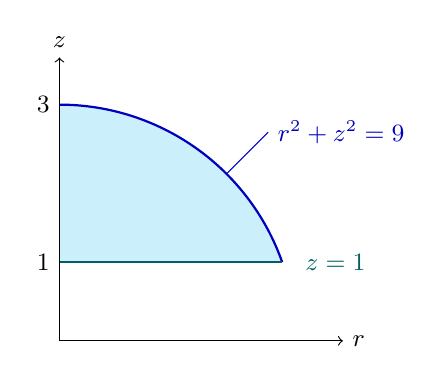
\begin{tikzpicture}[every node/.style={font=\small}]
    \fill[cyan!20] (0,1) -- (0,3)
        arc[start angle=90,end angle=19.47122,radius=3] -- cycle;
    \draw[blue!75!black,thick] (0,3)
        arc[start angle=90,end angle=19.47122,radius=3];
    \draw[teal!75!black,thick] (0,1) -- ({sqrt(8)},1);
    \draw[->] (0,0) -- (3.6,0) node[right] {$r$};
    \draw[->] (0,0) -- (0,3.6) node[above] {$z$};
    \node[left] at (0,1) {$1$};
    \node[left] at (0,3) {$3$};
    \node[right,teal!75!black] at (3,1) {$z=1$};
    \draw[blue!75!black] (2.12,2.12) -- (2.65,2.65)
        node[right] {$r^2+z^2=9$};
\end{tikzpicture}
\end{center}
\endgroup
